% !TeX root = RJwrapper.tex
\title{treeSS: Tree-Spatial Scan Statistic for Cluster Detection in R}


\author{by Allan Quadros, André L. F. Cançado, Geiziane S. Oliveira, and Luiz H. Duczmal}

\maketitle

\abstract{%
We introduce \textbf{treeSS}, an R package implementing the tree-spatial scan statistic of Cançado et al.~(2025). The method generalizes Kulldorff's circular spatial scan statistic by searching jointly over circular spatial zones and branches of a hierarchical classification tree, returning the (zone, branch) pair that maximizes the likelihood ratio under either a Poisson or a binomial model. Significance is assessed via Monte Carlo simulation against the null distribution of the maximum statistic over the entire (zone, branch) search space, so the family-wise error rate is controlled by construction regardless of the size of the tree or the number of candidate spatial zones. The joint scan recovers cause-specific signal that purely spatial scans miss when the rest of the study area is dominated by other causes, and the maximum-likelihood cut tends to be the clinically specific node rather than the most aggregated parent, which makes the output directly actionable in surveillance practice. The package targets epidemiological and surveillance applications where the events to be clustered carry both a geographic location and a categorical hierarchy, such as deaths classified by ICD-10, crimes by FBI category, or road collisions by severity. No previous CRAN package implements this combined scan; existing tools cover either spatial-only scans (such as \textbf{SpatialEpi}), space-time scans (such as \textbf{scanstatistics}), or wrappers around external binaries (such as \textbf{rsatscan} for SaTScan). The core search is implemented in C++ via \textbf{Rcpp} and optionally parallelized with OpenMP. We illustrate the package on three real datasets shipped with it -- infant mortality in Rio de Janeiro state (Brazil), reported crimes in Chicago community areas, and road traffic collisions across the 33 boroughs of London -- and show that the package reproduces the results reported in the original methodology paper.
}

\hypertarget{introduction}{%
\section{Introduction}\label{introduction}}

Detecting unusual clusters of events in space is a long-standing problem in
public-health surveillance, criminology, ecology, and demography. The
canonical tool is Kulldorff's circular spatial scan statistic
\citep{kulldorff1995, kulldorff1997}, implemented in the standalone SaTScan
software \citep{satscan} and widely used to identify localized excess risk in
disease incidence, mortality, and crime rates. Within R, the scan statistic
is exposed through several packages of varying scope: \CRANpkg{SpatialEpi}
\citep{spatialepi} provides Kulldorff's circular scan, \CRANpkg{scanstatistics}
\citep{scanstatistics} focuses on space-time anomaly detection, and
\CRANpkg{rsatscan} \citep{rsatscan} offers a thin wrapper around the SaTScan
binary, requiring an external installation.

A complementary line of work treats the events themselves as carrying
\emph{hierarchical} structure rather than spatial structure. The tree-based scan
statistic of \citet{kulldorff2003} was developed for adverse-event surveillance,
where events (such as drug-related diagnoses) are classified into a tree
(such as ICD chapters, subchapters, and leaf codes), and the goal is to
identify a \emph{branch} of the tree showing excess risk relative to its
expectation. The reference implementation, TreeScan \citep{treescan}, is again a
standalone binary; no CRAN package implements this method directly.

In many applied settings the two structures coexist. Infant deaths are
indexed by both \emph{municipality} (a spatial location) and \emph{ICD-10 cause} (a
position in a disease tree). Reported crimes are indexed by both
\emph{neighborhood} and \emph{offense category} (a hierarchy of theft, assault,
property crime, and so on). Road traffic collisions are indexed by both
\emph{borough} and \emph{severity ladder}. A purely spatial scan would aggregate over
all causes and miss a cause-specific cluster confined to a region; a purely
tree-based scan would aggregate over the whole study area and miss the
geographic concentration of a particular cause. The cluster of interest, in
each case, is a (region set, tree branch) pair.

\citet{cancado2025} introduced a \emph{tree-spatial scan statistic} that searches for
exactly such pairs. For each circular spatial zone \(z\) in the sense of
\citet{kulldorff1997} and each branch \(g\) of a user-supplied tree, the statistic
computes the likelihood ratio comparing a model where events in \((z, g)\)
follow an elevated Poisson (or binomial) rate against the null of a uniform
rate, and reports the pair maximizing this ratio. Significance is assessed
by Monte Carlo simulation under the null. The method was validated on
infant mortality data from the state of Rio de Janeiro, where it identified
a previously undocumented cluster of deaths classified as ICD-10 P20.9
(unspecified intrauterine hypoxia) concentrated in the north of the state.

The joint search has three properties that motivate it over running a
spatial scan and a tree-based scan separately and reconciling the outputs.
First, \emph{family-wise error rate (FWER) is controlled by construction}. The
Monte Carlo \(p\)-value is computed against the null distribution of the
maximum statistic over the \emph{entire} (zone, branch) search space, so the
test is exact regardless of how many candidate cuts and zones the
algorithm considers internally. By contrast, applying a tree-only scan and
declaring every cut with \(p < \alpha\) to be a finding, as \citet{kulldorff2003}
do for the same Rio de Janeiro data, returns more than fifty significant
ICD-10 cuts at the 5\% level \citep[Table 6]{cancado2025} -- a result of
multiple testing across tree branches that the user must then correct
manually. The tree-spatial scan returns one most-likely (zone, branch)
pair with one \(p\)-value, and the package then exposes principled
distinct-secondary-cluster procedures (Section \ref{sec-methodology}) on
top of that single test. Second, \emph{the joint scan recovers cause-specific
signal that pure-spatial scans miss}. On the Rio de Janeiro data the
purely spatial scan locates a 8-municipality cluster around the state
capital driven by the aggregate death count \citep[Table 5]{cancado2025}; the
joint scan additionally identifies an 18-municipality cluster of P20.9
deaths in the north fluminense region with relative risk approximately
\(8\times\) -- a signal that aggregate-counts-only methods cannot resolve
because the rest of the state is dominated by other causes. Third, \emph{the
maximum-likelihood cut tends to be the clinically specific node, not the
most aggregated parent}. In the Rio de Janeiro analysis the joint scan
returns the leaf P20.9 rather than its parent chapter (P00--P96, all
perinatal conditions), even though the parent contains many more events,
because the likelihood ratio penalizes dilution of effect across
heterogeneous siblings. This property makes the output directly
actionable for surveillance practice.

This paper introduces \CRANpkg{treeSS}, an R package implementing this
method. To our knowledge it is the first CRAN package providing a
tree-spatial scan; \CRANpkg{scanstatistics} does not address the tree
dimension, \CRANpkg{rsatscan} delegates to a binary that does not implement
this combined scan, and the standalone TreeScan software does not perform
the spatial search. The package additionally provides standalone
implementations of the circular spatial scan \citep{kulldorff1997} and the
tree-based scan \citep{kulldorff2003} under a unified interface, so that the
three scan types -- spatial-only, tree-only, and tree-spatial -- can be
compared on the same data with the same input contract. The likelihood-ratio
search and the Monte Carlo loop are implemented in C++ via \CRANpkg{Rcpp}
\citep{rcpp} and optionally parallelized with OpenMP \citep{openmp}, yielding a
4--8\(\times\) speedup on multicore machines. Three real datasets are shipped
with the package -- infant mortality in Rio de Janeiro \citep{datasus, ibge},
reported crime in Chicago \citep{chicagoportal}, and road traffic collisions in
London \citep{stats19} -- to allow users to run the full workflow end-to-end
without preparing data themselves.

The remainder of this paper is structured as follows. Section
\ref{sec-methodology} summarizes the methodology to the level needed for
the rest of the paper, deferring derivations and proofs to \citet{cancado2025}.
Section \ref{sec-design} describes the package design, with particular
attention to the choice of input contract, the class hierarchy of scan
results, and the helper functions for cluster extraction and visualization.
Section \ref{sec-example} walks through a complete worked example
reproducing the results of \citet{cancado2025} on the Rio de Janeiro infant
mortality data. Section \ref{sec-applications} gives two further
applications, on the Chicago crime and London collisions datasets, to
illustrate the breadth of the method. Section \ref{sec-implementation}
discusses implementation details, performance, and limitations. Section
\ref{sec-comparison} compares \textbf{treeSS} with related packages and
standalone tools. We conclude in Section \ref{sec-discussion}.

\hypertarget{sec-methodology}{%
\section{Methodology overview}\label{sec-methodology}}

This section sketches just enough of the tree-spatial scan statistic to make
the rest of the paper self-contained. For full derivations, the choice of
significance procedure, and simulation studies, we refer the reader to
\citet{cancado2025}.

\textbf{Setup.} Let \(i = 1, \ldots, m\) index the regions of a study area, with
populations \(n_i\) and centroids \((x_i, y_i)\). Let \(T\) be a rooted tree whose
leaves \(\ell\) enumerate the categories that observed events fall into, and
whose internal nodes represent aggregations of those categories. We denote
by \(L(g) \subseteq \{\ell\}\) the set of leaves in the subtree rooted at
node \(g\). The data are integer counts \(c_{i,\ell}\) of events occurring in
region \(i\) and classified into leaf \(\ell\). Writing \(C = \sum_{i,\ell} c_{i,\ell}\) for the total event count and \(N = \sum_i n_i\) for the total
population, the count rolled up to a tree branch \(g\) is
\(C_g = \sum_i \sum_{\ell \in L(g)} c_{i,\ell}\), and the count restricted to
both a zone \(z \subseteq \{1,\ldots,m\}\) and a branch \(g\) is
\(c_{z,g} = \sum_{i \in z} \sum_{\ell \in L(g)} c_{i,\ell}\) with population
\(n_z = \sum_{i \in z} n_i\).

\textbf{Spatial zones.} Following \citet{kulldorff1997}, the family of candidate zones
\(\mathcal{Z}\) consists of circular zones: for each region \(i\) (the center)
and each \(k = 1, 2, \ldots\), the zone \(z_{i,k}\) is the union of the \(k\)
regions nearest to \(i\) in Euclidean distance between centroids, capped at a
maximum population fraction (default \(50\%\) of \(N\)). This produces of order
\(O(m^2)\) candidate zones with limited combinatorial blow-up.

\textbf{Likelihood ratio.} Under a Poisson model, the log likelihood ratio for
a single (zone, branch) pair \((z, g)\) is

\[
\Lambda(z, g) =
c_{z,g} \log \frac{c_{z,g}}{\mathbb{E}[c_{z,g}]} +
(C_g - c_{z,g}) \log \frac{C_g - c_{z,g}}{C_g - \mathbb{E}[c_{z,g}]}
\quad \text{if } c_{z,g} > \mathbb{E}[c_{z,g}],
\]

and \(0\) otherwise, where \(\mathbb{E}[c_{z,g}] = C_g \cdot n_z / N\) is the
expected count in \((z, g)\) under uniform risk. Under a binomial model -- in
which \(n_i\) counts trials rather than population at risk -- the
corresponding expression replaces Poisson rates by binomial proportions; we
omit the formula for brevity (see \citet{cancado2025}, eq. 4). The tree-spatial
scan statistic is

\[
\Lambda^* = \max_{z \in \mathcal{Z}, \, g \in T} \Lambda(z, g),
\]

and the \emph{most likely cluster} is the maximizing pair.

\textbf{Inference.} No tractable null distribution is available for \(\Lambda^*\).
Following \citet{kulldorff1997}, significance is assessed by Monte Carlo
simulation: under \(H_0\), the observed leaf-by-region count matrix is
re-sampled from a multinomial distribution conditional on the row totals
\(C_\ell\) (the leaf marginals) and on the population shares \(n_i / N\), the
statistic is recomputed on each replicate, and the \(p\)-value of \(\Lambda^*\)
is the rank of the observed value among the simulated maxima. Because the
test statistic is the \emph{maximum} of \(\Lambda(z, g)\) over the entire
candidate space and the simulated null is the distribution of that same
maximum, the resulting \(p\)-value is exact regardless of how many candidate
zones and branches the algorithm sweeps over -- the family-wise error rate
is controlled by construction. This is what makes the joint scan
preferable to running a tree-only scan and applying multiple-testing
corrections after the fact: in the latter case, with thousands of
candidate cuts in a realistic ICD-10 tree, even the \citet{holm1979} correction
produces a very conservative test, whereas the joint Monte Carlo \(p\)-value
needs no post-hoc adjustment.

\textbf{Secondary clusters.} The most likely cluster is rarely the only signal
of interest. \citet{cancado2025}, Section 5.1.1, retains additional (zone, branch)
pairs in decreasing order of \(\Lambda\), declaring a candidate \emph{distinct}
from those already retained when its branch is neither an ancestor nor a
descendant of any retained branch, \emph{or} its zone has no region in common
with any retained zone. Section \ref{sec-design} below describes how this
is exposed in \textbf{treeSS} through the \texttt{filter\_clusters()} and
\texttt{get\_cluster\_regions()} helpers. We additionally provide a sequential
\emph{conditional} procedure inspired by \citet{zhang2010} in \texttt{iterative\_scan()},
which is not part of the original paper and is offered as a complementary
tool for users who prefer Holm--Bonferroni-corrected sequential testing.

The three scans -- circular spatial, tree, tree-spatial -- share this
template. The spatial-only case takes a degenerate single-leaf tree and
reduces to \citet{kulldorff1997}. The tree-only case takes a degenerate
single-region geography and reduces to \citet{kulldorff2003}. The package exposes
all three via a unified interface, described next.

\hypertarget{sec-design}{%
\section{Package design}\label{sec-design}}

The interface of \textbf{treeSS} was shaped by three observations from the
applied workflows we have in mind. First, scan-statistic inputs are
heterogeneous: per-region counts and populations, per-region centroids,
per-event leaf labels, and a tree structure that lives outside the
case-level table. Second, the choice of denominator (resident population
vs.~live births vs.~number of trials) is a substantive scientific decision
in surveillance work, and the package should make that decision explicit
rather than infer it from column names. Third, users will mix the three
scan types -- spatial-only, tree-only, and tree-spatial -- on the same
data, so the three functions should share an input contract and a result
schema. The subsections below describe how these observations translate
into concrete API choices.

\hypertarget{input-contract-parallel-vectors}{%
\subsection{Input contract: parallel vectors}\label{input-contract-parallel-vectors}}

A scan-statistic call has many distinct inputs: per-region case counts and
populations, per-region centroids, the leaf classification of each event,
the tree structure itself, the model, the number of simulations, and the
significance threshold. Three input designs were considered:

\begin{enumerate}
\def\labelenumi{\arabic{enumi}.}
\tightlist
\item
  \textbf{A single \texttt{data.frame}} with reserved column names. This is the style
  used by SaTScan input files. It is concise but ambiguous when the user's
  data has columns with different names: the user must rename, or the
  package must guess.
\item
  \textbf{A formula interface}, in the style of \texttt{lm()}. This works well when
  inputs are scalars per row, but a tree-spatial scan needs tree
  structure as a side input that does not fit into a formula naturally.
\item
  \textbf{Parallel vectors}, one per logical role.
\end{enumerate}

We chose the third. Every scan function in \textbf{treeSS} accepts the
case-level inputs as named, parallel vectors:

\begin{verbatim}
treespatial_scan(
  cases, population, region_id, x, y, node_id,
  tree = ..., ...
)
\end{verbatim}

Each role is named explicitly. The user picks which column of their data is
the denominator (for instance \texttt{live\_births} rather than the resident
\texttt{population}, when computing infant mortality rates). There is no implicit
column-name convention to memorise, and partial inputs are caught at call
time rather than mid-scan. The cost is verbosity: a typical call has six
to eight named arguments. We consider that an acceptable price for an
explicit, auditable interface, especially in surveillance contexts where
the choice of denominator is a substantive scientific decision.

The tree itself can be supplied either as a two-column \texttt{data.frame} with
columns \texttt{node\_id} and \texttt{parent\_id} (root having \texttt{parent\_id\ =\ NA}), or as
two parallel vectors \texttt{tree\_node\_id} and \texttt{tree\_parent\_id}. The two forms
are interconvertible, so users can use whichever fits their preprocessing.

\hypertarget{function-hierarchy}{%
\subsection{Function hierarchy}\label{function-hierarchy}}

The package exposes three scan functions, an iterative wrapper, two
post-processing helpers, and one tree-construction helper. Table
\ref{tab:functions} summarizes them.

\begin{table}

\caption{\label{tab:functions}User-facing functions in the treeSS package.}
\centering
\begin{tabular}[t]{ll}
\toprule
Function & Purpose\\
\midrule
treespatial\_scan() & Tree-spatial scan; main entry point\\
circular\_scan() & Kulldorff's circular spatial scan, no tree\\
tree\_scan() & Tree-based scan, no spatial dimension\\
iterative\_scan() & Sequential conditional scan with Holm--Bonferroni correction\\
filter\_clusters() & Distinct secondary clusters per Cançado et al. (2025), Sec. 5.1.1\\
\addlinespace
get\_cluster\_regions() & Tidy region-by-cluster table for plotting\\
aggregate\_tree() & Roll counts up the tree to internal nodes\\
build\_zones() & Construct the family of circular zones\\
\bottomrule
\end{tabular}
\end{table}

The first three functions return objects of S3 classes
\texttt{"treespatial\_scan"}, \texttt{"circular\_scan"}, and \texttt{"tree\_scan"}, respectively;
\texttt{iterative\_scan()} returns an object of class \texttt{"iterative\_scan"}. Every
class has \texttt{print()} and \texttt{summary()} methods, and \texttt{get\_cluster\_regions()} is
an S3 generic with a default method (single-pass scans) and a dedicated
method for \texttt{"iterative\_scan"} objects, allowing the same downstream
visualization pipeline regardless of which scan was used.

\hypertarget{choice-of-model-poisson-and-binomial}{%
\subsection{Choice of model: Poisson and binomial}\label{choice-of-model-poisson-and-binomial}}

All scan functions accept \texttt{model\ =\ c("poisson",\ "binomial")}, defaulting
to Poisson. The choice changes the form of the likelihood ratio
(Section \ref{sec-methodology}) but not the search procedure or the
Monte Carlo step. The Poisson model is appropriate when the denominator
is a \emph{population at risk} and case rates are small, which is the typical
surveillance setting. The binomial model is appropriate when the
denominator is a \emph{number of trials} (cases-plus-controls), as in
case-control studies of rare adverse events.

\hypertarget{parallel-monte-carlo}{%
\subsection{Parallel Monte Carlo}\label{parallel-monte-carlo}}

The Monte Carlo step is the dominant cost: each replicate re-runs the full
\(O(|\mathcal{Z}| \cdot |T|)\) likelihood evaluation. All scan functions
expose \texttt{n\_cores} (default \texttt{1L}); when \texttt{n\_cores\ \textgreater{}\ 1}, replicates are
distributed across OpenMP threads in C++. Each thread carries its own
\texttt{std::mt19937} generator seeded deterministically from the user-supplied
\texttt{seed}. Two reproducibility properties hold:

\begin{itemize}
\tightlist
\item
  \texttt{n\_cores\ =\ 1} is bit-identical to the pre-OpenMP serial implementation.
\item
  \texttt{n\_cores\ \textgreater{}\ 1} is reproducible for any fixed pair \texttt{(seed,\ n\_cores)},
  but differs slightly from the serial path because R's RNG cannot be
  shared across threads safely; the simulated null distribution comes from
  the thread-local Mersenne Twister streams.
\end{itemize}

For publication-critical work where the simulated \(p\)-values must be
bit-identical between machines, we recommend \texttt{n\_cores\ =\ 1L}. For
exploratory work, \texttt{n\_cores\ =\ 4} typically yields a 4--6\(\times\) speedup
(see Section \ref{sec-implementation}).

\hypertarget{result-objects}{%
\subsection{Result objects}\label{result-objects}}

Each scan returns a list with a stable schema. For
\texttt{treespatial\_scan()}:

\begin{longtable}[]{@{}
  >{\raggedright\arraybackslash}p{(\columnwidth - 2\tabcolsep) * \real{0.5000}}
  >{\raggedright\arraybackslash}p{(\columnwidth - 2\tabcolsep) * \real{0.5000}}@{}}
\toprule()
\begin{minipage}[b]{\linewidth}\raggedright
Element
\end{minipage} & \begin{minipage}[b]{\linewidth}\raggedright
Description
\end{minipage} \\
\midrule()
\endhead
\texttt{most\_likely\_cluster} & List with \texttt{node\_id}, \texttt{region\_ids}, \texttt{cases}, \texttt{expected}, \texttt{population}, \texttt{rr}, \texttt{llr} \\
\texttt{secondary\_clusters} & Data.frame of all (zone, branch) pairs evaluated, sorted by LLR \\
\texttt{pvalue} & Monte Carlo \(p\)-value for the most likely cluster \\
\texttt{nsim}, \texttt{alpha}, \texttt{model} & Hyperparameters passed in by the user \\
\texttt{simulated\_llr} & Vector of length \texttt{nsim} with the simulated null distribution \\
\texttt{regions}, \texttt{tree}, \texttt{full\_cases} & Inputs preserved for downstream use \\
\bottomrule()
\end{longtable}

The \texttt{secondary\_clusters} table makes the post-processing functions
\texttt{filter\_clusters()} and \texttt{get\_cluster\_regions()} cheap: no additional Monte
Carlo simulation is required to extract distinct clusters of arbitrary
rank. The user pays for the simulation once, then explores the result
interactively.

\hypertarget{datasets}{%
\subsection{Datasets}\label{datasets}}

The package ships three real datasets, each accompanied by its tree and
(where applicable) a polygon layer for visualization. Table
\ref{tab:datasets} summarizes them. They were chosen to span three
different domains, three different denominator conventions, and three
different tree sizes, so that users encountering the method can find an
example structurally similar to their own.

\begin{table}

\caption{\label{tab:datasets}Real-world datasets shipped with treeSS. The regions column reports the number of spatial units. Each dataset is paired with a corresponding tree object.}
\centering
\begin{tabular}[t]{lllll}
\toprule
Dataset & Country & Domain & Regions & Tree (nodes)\\
\midrule
rj\_mortality & Brazil & Health & 89 & ICD-10 (622)\\
chicago\_crimes & USA & Crime & 77 & Crime taxonomy (2841)\\
london\_collisions & UK & Road safety & 33 & Conditions (81)\\
\bottomrule
\end{tabular}
\end{table}

A fourth dataset, \texttt{fl\_deaths}, ships in raw long form -- 65 Florida
counties, 253 ICD-10 codes, \textasciitilde157,000 deaths in 2016 -- and is intended as
a pedagogical exercise in which the user constructs the tree and the
case matrix from scratch. It is exercised in
\texttt{inst/examples/example\_florida.R}.

\hypertarget{sec-example}{%
\section{Worked example: replicating Cançado et al.~(2025)}\label{sec-example}}

We reproduce Section 5.2 of \citet{cancado2025}, the analysis of infant deaths in
Rio de Janeiro state in 2016. The dataset, \texttt{rj\_mortality}, contains
counts of infant deaths in 89 of the state's 92 municipalities, classified
by 4-character ICD-10 leaf codes. The tree, \texttt{rj\_tree}, is the ICD-10
hierarchy with 622 nodes and 410 leaves. The denominator for an
infant-mortality rate analysis is \texttt{live\_births}, the number of registered
live births in 2016 (DATASUS/SINASC).

\begin{verbatim}
library(treeSS)
data(rj_mortality)
data(rj_tree)

c(rows = nrow(rj_mortality),
  municipalities = length(unique(rj_mortality$region_id)),
  tree_nodes = nrow(rj_tree),
  total_deaths = sum(rj_mortality$cases),
  total_births = sum(unique(rj_mortality[, c("region_id", "live_births")])$live_births))
#>           rows municipalities     tree_nodes   total_deaths 
#>           1440             89            622           2981 
#>   total_births 
#>         218759
\end{verbatim}

The scan is one function call:

\begin{verbatim}
result_rj <- treespatial_scan(
  cases       = rj_mortality$cases,
  population  = rj_mortality$live_births,
  region_id   = rj_mortality$region_id,
  x           = rj_mortality$x,
  y           = rj_mortality$y,
  node_id     = rj_mortality$node_id,
  tree        = rj_tree,
  max_pop_pct = 0.50,
  nsim        = 999, seed = 2016, n_cores = 4L
)
print(result_rj)
#> Tree-Spatial Scan Statistic
#> -------------------------------------------------- 
#> Total population: 218759 
#> Number of regions: 89 
#> Number of tree nodes: 622 
#> Monte Carlo simulations: 999 
#> 
#> Most likely cluster:
#>   Tree node: P209 
#>   Leaf IDs: P209
#> 
#>   Regions: 71, 74, 19, 17, 31, 11, 72, 62, 14, 33, ... and 8
#>            more
#> 
#>   Number of regions: 18 
#>   Cases in (zone, branch): 27 
#>   Expected: 3.34 
#>   Population: 12604 
#>   Relative risk: 8.0797 
#>   Log-LR: 38.8319 
#>   P-value: 0.001
\end{verbatim}

The most likely cluster is the ICD-10 leaf code \textbf{P209} (``Unspecified
intrauterine hypoxia'') concentrated in 18 contiguous municipalities of
the north fluminense region. Twenty-seven deaths are observed against an
expectation of approximately 3.34 under uniform risk -- a relative risk of
\(\sim 8\times\) -- with a Monte Carlo \(p\)-value below \(1/(\text{nsim}+1)\).
This matches Table 7 of \citet{cancado2025}: the same 18 municipalities (by IBGE
code), 27 observed deaths, expected \(\approx 3.37\), log-likelihood ratio
\(LR = 38.48\) (we obtain \(\approx 38.83\)). The minor LR discrepancy is
explained in \citet{cancado2025} by a SIM database update post-2016 and by the
discontinuation of TCU population estimates after 2017; the conclusions
are identical.

To make the value of the joint scan concrete, it is worth running the
two simpler scans on exactly the same data. The purely \emph{spatial} scan,
ignoring the tree, returns a single 8-municipality cluster around
greater Rio de Janeiro driven by the aggregate death count
\citep[Table 5]{cancado2025}; the P209 cluster in the north of the state
does not appear at all, because aggregating over all causes dilutes the
cause-specific signal. We can verify this directly by aggregating
\texttt{rj\_mortality} to one row per municipality and running the circular
scan on the totals:

\begin{verbatim}
# Aggregate cases to one row per municipality.
rj_agg <- unique(rj_mortality[, c("region_id", "x", "y", "live_births")])
rj_agg$cases <- tapply(rj_mortality$cases,
                       rj_mortality$region_id,
                       sum)[as.character(rj_agg$region_id)]
rj_agg <- rj_agg[order(rj_agg$region_id), ]

result_rj_spatial <- circular_scan(
  cases       = rj_agg$cases,
  population  = rj_agg$live_births,
  region_id   = rj_agg$region_id,
  x           = rj_agg$x,
  y           = rj_agg$y,
  max_pop_pct = 0.50,
  nsim        = 999, seed = 2016, n_cores = 4L
)
result_rj_spatial$most_likely_cluster$region_ids
#>  [1] 72 14 31 32 19 76 69  2 79 17 70
\end{verbatim}

Conversely, the purely \emph{tree-based} scan, ignoring geography, returns more
than fifty significant cuts at the 5\% level on this dataset
\citep[Table 6]{cancado2025}; the analyst is then left to apply a
multiple-testing correction across tree branches and to decide which
findings to follow up. The joint scan returns a \emph{single} most-likely
\((z, g)\) pair with one Monte Carlo \(p\)-value -- the family-wise error
rate is already controlled by the joint maximization, and Section
\ref{sec-distinct-secondary} below shows how distinct secondary
clusters are extracted from the same fit at no additional Monte Carlo
cost.

\hypertarget{sec-distinct-secondary}{%
\subsection{Distinct secondary clusters}\label{sec-distinct-secondary}}

The original paper reports more than one cluster per scan, using the
Section 5.1.1 procedure: pairs are retained in decreasing \(\Lambda\) as long
as they are \emph{distinct} from those already retained. \textbf{treeSS} exposes
this directly via \texttt{filter\_clusters()}:

\begin{verbatim}
fc <- filter_clusters(result_rj)
head(fc[, c("node_id", "n_regions", "cases", "expected", "llr", "pvalue")], 5)
#>        node_id n_regions cases  expected      llr pvalue
#> 859767    P209        18    27  3.341723 38.83194  0.001
#> 527361    Ch_X        18   118 74.410996 17.84292  0.001
#> 105806    W849         6    35 14.622475 14.15378  0.007
#> 762910     P23         8     9  1.068683 13.48971  0.016
#> 105264    P361         3     5  0.361768 13.13095  0.026
\end{verbatim}

No additional Monte Carlo simulation is performed; the secondary clusters
are read from \texttt{result\_rj\$secondary\_clusters} and filtered for distinctness
in \(O(k^2)\) time, where \(k\) is the number of clusters requested. The
top filtered candidates correspond to the rows of Table 7 of
\citet{cancado2025}.

\hypertarget{visualizing-the-cluster}{%
\subsection{Visualizing the cluster}\label{visualizing-the-cluster}}

\texttt{get\_cluster\_regions()} returns a tidy data.frame mapping each region to
each retained cluster, ready to merge with a polygon layer. The package
does not ship \texttt{sf} polygons for Rio de Janeiro -- they are easy to fetch
on demand from \CRANpkg{geobr}:

\begin{verbatim}
library(ggplot2)
library(geobr)
library(sf)
library(dplyr)

rj_map <- read_municipality(code_muni = "RJ", year = 2016,
                            showProgress = FALSE)
rj_map$code6 <- as.integer(substr(rj_map$code_muni, 1, 6))
ibge_lookup <- unique(rj_mortality[, c("region_id", "ibge_code")])
\end{verbatim}

\begin{verbatim}
mlc_rj <- result_rj$most_likely_cluster
cr_rj_1 <- merge(
  get_cluster_regions(result_rj, n_clusters = 1L, overlap = FALSE),
  ibge_lookup, by = "region_id"
)

# Join cluster-membership data into the polygon layer. We use the
# sf-aware `dplyr::left_join.sf` method directly, which preserves
# geometry across rows even when the right-hand-side data.frame has
# duplicate join keys (as it does for cr_rj_2 below, which has 2 rows
# per region under overlap = TRUE). This is the pattern used in the
# official `geobr` vignette.
rj_p1 <- left_join(rj_map, cr_rj_1, by = c("code6" = "ibge_code"))

ggplot(rj_p1) +
  geom_sf(aes(fill = factor(cluster)), color = "gray40",
          linewidth = 0.15, alpha = 0.80) +
  scale_fill_manual(
    values   = c("1" = "#C44E52"), na.value = "gray95",
    na.translate = FALSE,
    labels   = paste0(mlc_rj$node_id, " (",
                      length(mlc_rj$region_ids), " municipalities)"),
    name     = "Cluster"
  ) +
  labs(subtitle = sprintf("LR = %.1f, p = %s | %d deaths (expected %.1f)",
                          mlc_rj$llr,
                          format.pval(result_rj$pvalue, digits = 3),
                          mlc_rj$cases, mlc_rj$expected)) +
  theme_minimal(base_size = 13) +
  theme(plot.subtitle = element_text(color = "gray35", size = 11),
        axis.title    = element_blank(),
        axis.text     = element_text(color = "gray55", size = 9))
\end{verbatim}

\begin{figure}

{\centering 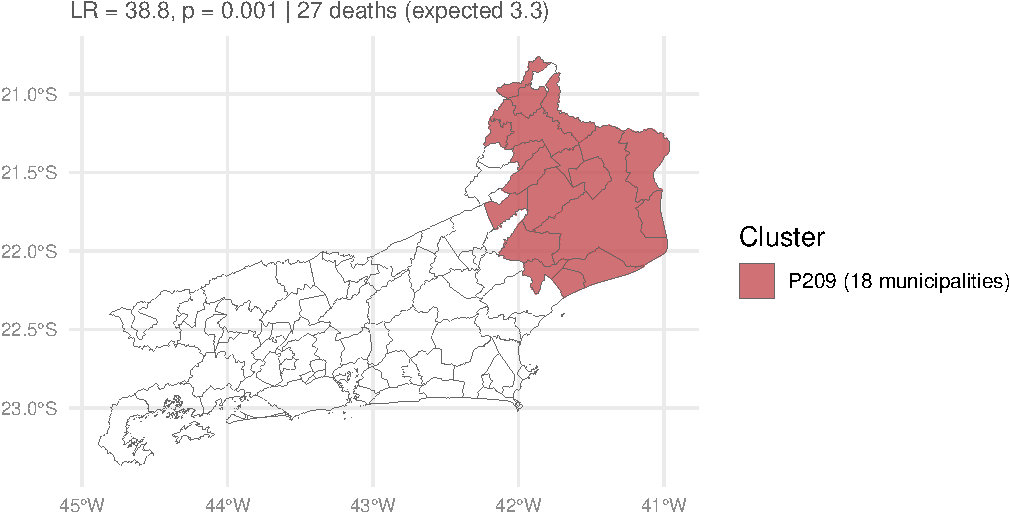
\includegraphics[width=0.9\linewidth]{treeSS_files/figure-latex/rj-plot-primary-1} 

}

\caption{Most likely tree-spatial cluster in Rio de Janeiro: 18 contiguous municipalities (red) of the north fluminense region with elevated mortality from ICD-10 P209 (unspecified intrauterine hypoxia). LR = 38.83, p < 0.001, 27 deaths observed against 3.34 expected.}\label{fig:rj-plot-primary}
\end{figure}

The same \texttt{get\_cluster\_regions()} call with \texttt{n\_clusters\ =\ 2,\ overlap\ =\ TRUE}
and the panel column produced by the helper drives a faceted plot
showing the most likely cluster alongside the top \emph{distinct} secondary
cluster according to the procedure of \citet{cancado2025}, Section 5.1.1
(i.e., whose branch is neither an ancestor nor a descendant of the
primary's branch, \emph{or} whose zone shares no region with the primary's
zone). No additional Monte Carlo simulation is run; the candidates are
read from \texttt{result\_rj\$secondary\_clusters}.

\begin{verbatim}
cr_rj_2 <- merge(
  get_cluster_regions(result_rj, n_clusters = 2L, overlap = TRUE),
  ibge_lookup, by = "region_id"
)

rj_p2 <- left_join(rj_map, cr_rj_2, by = c("code6" = "ibge_code"))

ggplot(rj_p2[!is.na(rj_p2$panel), ]) +
  geom_sf(aes(fill = factor(cluster)), color = "gray40",
          linewidth = 0.12, alpha = 0.80) +
  scale_fill_manual(values = c("1" = "#C44E52", "2" = "#4C72B0"),
                    na.value = "gray95", na.translate = FALSE) +
  facet_wrap(~ panel, nrow = 1L) +
  theme_minimal(base_size = 12) +
  theme(strip.text = element_text(face = "bold", size = 11),
        axis.title = element_blank(),
        axis.text  = element_text(color = "gray55", size = 9),
        legend.position = "none")
\end{verbatim}

\begin{figure}

{\centering 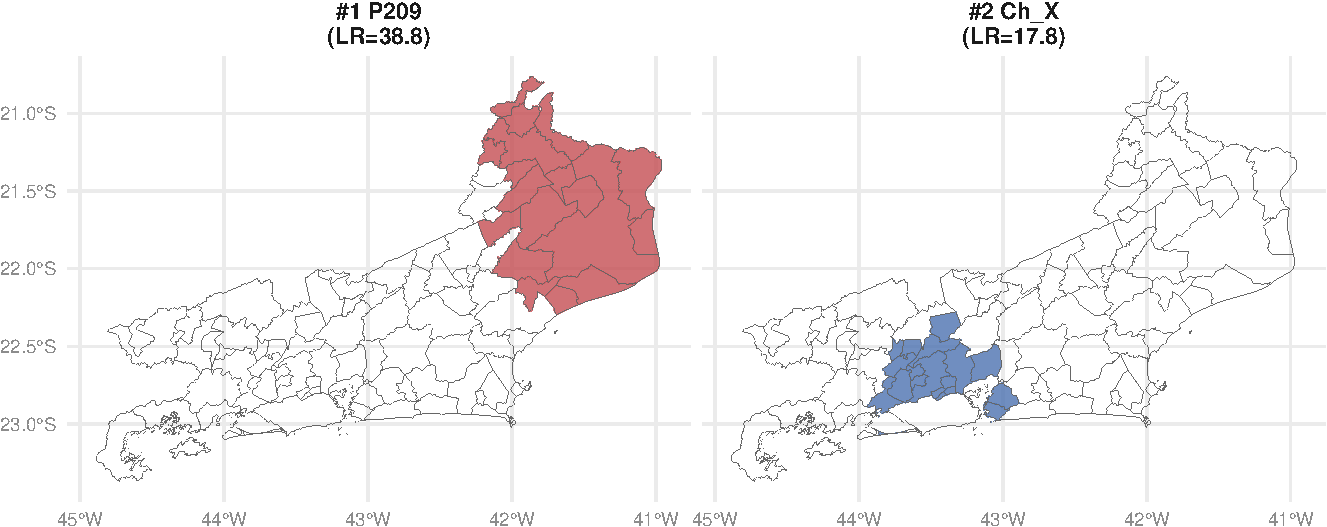
\includegraphics[width=0.9\linewidth]{treeSS_files/figure-latex/rj-plot-top2-1} 

}

\caption{Top-2 distinct tree-spatial clusters in Rio de Janeiro per Cançado et al. (2025), Section 5.1.1: the primary cluster (P209, north fluminense) and the highest-LR distinct secondary cluster.}\label{fig:rj-plot-top2}
\end{figure}

A complete annotated worked example is shipped at
\texttt{system.file("examples",\ "example\_brazil\_rj.R",\ package\ =\ "treeSS")}.

\hypertarget{sec-applications}{%
\section{Two further applications}\label{sec-applications}}

The second and third datasets exercise the same workflow on different
domains, denominator conventions, and tree sizes.

\hypertarget{reported-crimes-in-chicago-2023}{%
\subsection{Reported crimes in Chicago, 2023}\label{reported-crimes-in-chicago-2023}}

\texttt{chicago\_crimes} records \textasciitilde250,000 crime incidents across the 77 community
areas of Chicago in 2023, classified by a 2841-node tree of FBI primary
type, secondary description, and location category. The dataset ships with
two denominator columns: \texttt{population}, the total \emph{incidents} in each area
(a compositional denominator), and \texttt{pop\_residential}, the area's
\emph{residential population} from ACS 2020 5-year estimates. Either is a
legitimate denominator and they answer different questions:
incidents-per-resident vs.~share-of-citywide-incidents. We use
\texttt{pop\_residential} for an incidence-rate analysis.

\begin{verbatim}
data(chicago_crimes)
data(chicago_tree)
data(chicago_map)

result_chi <- treespatial_scan(
  cases       = chicago_crimes$cases,
  population  = chicago_crimes$pop_residential,
  region_id   = chicago_crimes$region_id,
  x           = chicago_crimes$x,
  y           = chicago_crimes$y,
  node_id     = chicago_crimes$node_id,
  tree        = chicago_tree,
  max_pop_pct = 0.25,
  nsim        = 999, seed = 2023, n_cores = 4L
)
print(result_chi)
#> Tree-Spatial Scan Statistic
#> -------------------------------------------------- 
#> Total population: 2713037 
#> Number of regions: 77 
#> Number of tree nodes: 2841 
#> Monte Carlo simulations: 999 
#> 
#> Most likely cluster:
#>   Tree node: Root 
#>   Leaf IDs: ARSON | AGGRAVATED | AIRPORT, ARSON | AGGRAVATED |
#>             CTA_TRANSIT, ARSON | AGGRAVATED | HOTEL, ARSON |
#>             AGGRAVATED | MEDICAL, ARSON | AGGRAVATED | OTHER,
#>             ARSON | AGGRAVATED | RESIDENCE, ARSON |
#>               AGGRAVATED |
#>             RESTAURANT_BAR, ARSON | AGGRAVATED | RETAIL,
#>               ARSON |
#>             AGGRAVATED | SCHOOL, ARSON | ATTEMPT ARSON |
#>             COMMERCIAL, ... and 2476 more
#> 
#>   Regions: 46, 48, 43, 45, 52, 47, 51, 42, 50, 44, ... and 16
#>            more
#> 
#>   Number of regions: 26 
#>   Cases in (zone, branch): 85144 
#>   Expected: 53901.73 
#>   Population: 558595 
#>   Relative risk: 1.5796 
#>   Log-LR: 10158.85 
#>   P-value: 0.001
\end{verbatim}

The most likely cluster is a contiguous group of community areas on
Chicago's South Side -- Englewood, West Englewood, Auburn Gresham, Roseland
and immediate neighbors -- driven by an over-occurrence of violent and
property crimes against residents. The \textbf{treeSS} result is consistent
with the spatial pattern that Chicago's annual public-safety reports
describe; what is novel is that \textbf{treeSS} identifies the \emph{combination}
of crime category and geographic extent jointly, rather than running
separate spatial scans per category. Figure \ref{fig:chi-plot-primary}
shows the primary cluster; Figure \ref{fig:chi-plot-top2} shows the
top two distinct clusters retained by the procedure of \citet{cancado2025},
Section 5.1.1.

\begin{verbatim}
mlc_chi <- result_chi$most_likely_cluster
chi_lookup <- unique(chicago_crimes[, c("region_id", "area_number")])
cr_chi_1 <- merge(
  get_cluster_regions(result_chi, n_clusters = 1L, overlap = FALSE),
  chi_lookup, by = "region_id"
)
chi_p1 <- left_join(chicago_map, cr_chi_1,
                    by = c("AREA_NUM" = "area_number"))

ggplot(chi_p1) +
  geom_sf(aes(fill = factor(cluster)), color = "gray40",
          linewidth = 0.15, alpha = 0.80) +
  scale_fill_manual(
    values   = c("1" = "#C44E52"), na.value = "gray95",
    na.translate = FALSE,
    labels   = paste0(mlc_chi$node_id, " (",
                      length(mlc_chi$region_ids), " areas)"),
    name     = "Cluster"
  ) +
  labs(subtitle = sprintf("LR = %.1f, p = %s | %d incidents (expected %.1f)",
                          mlc_chi$llr,
                          format.pval(result_chi$pvalue, digits = 3),
                          mlc_chi$cases, mlc_chi$expected)) +
  theme_minimal(base_size = 13) +
  theme(plot.subtitle = element_text(color = "gray35", size = 11),
        axis.title    = element_blank(),
        axis.text     = element_text(color = "gray55", size = 9))
\end{verbatim}

\begin{figure}

{\centering 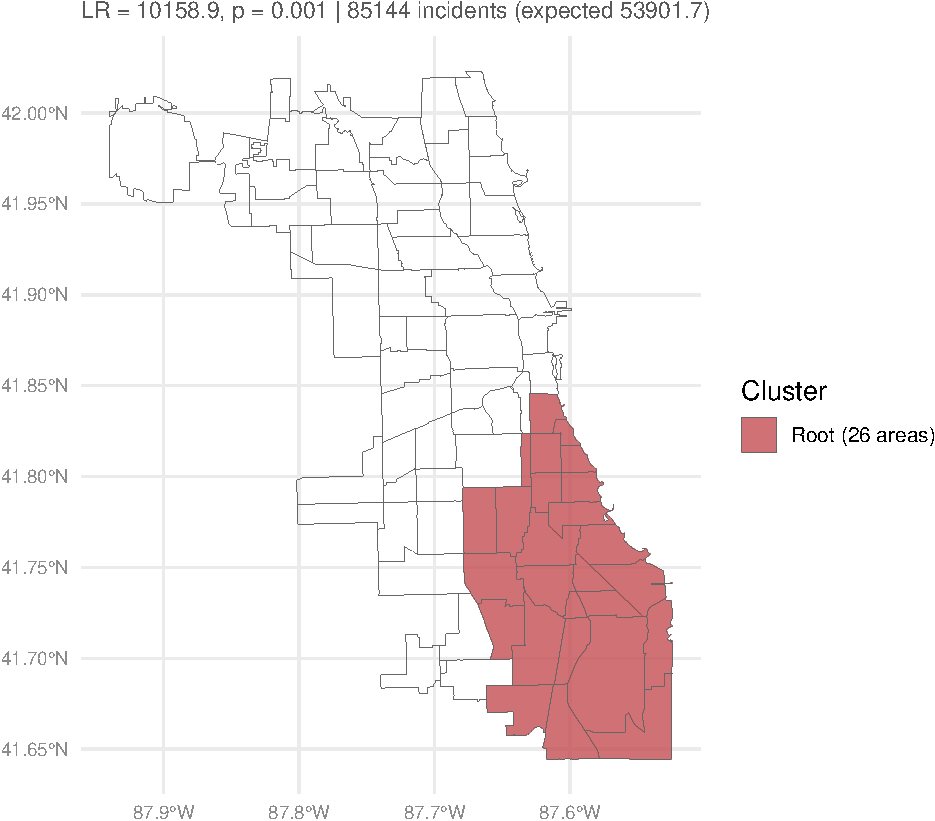
\includegraphics[width=0.9\linewidth]{treeSS_files/figure-latex/chi-plot-primary-1} 

}

\caption{Most likely tree-spatial cluster in Chicago, 2023: contiguous community areas on the South Side with elevated crime incidence. Denominator: residential population (ACS 2020 5-year).}\label{fig:chi-plot-primary}
\end{figure}

\begin{verbatim}
cr_chi_2 <- merge(
  get_cluster_regions(result_chi, n_clusters = 2L, overlap = TRUE),
  chi_lookup, by = "region_id"
)
chi_p2 <- left_join(chicago_map, cr_chi_2,
                    by = c("AREA_NUM" = "area_number"))

ggplot(chi_p2[!is.na(chi_p2$panel), ]) +
  geom_sf(aes(fill = factor(cluster)), color = "gray40",
          linewidth = 0.12, alpha = 0.80) +
  scale_fill_manual(values = c("1" = "#C44E52", "2" = "#4C72B0"),
                    na.value = "gray95", na.translate = FALSE) +
  facet_wrap(~ panel, nrow = 1L) +
  theme_minimal(base_size = 12) +
  theme(strip.text = element_text(face = "bold", size = 11),
        axis.title = element_blank(),
        axis.text  = element_text(color = "gray55", size = 9),
        legend.position = "none")
\end{verbatim}

\begin{figure}

{\centering 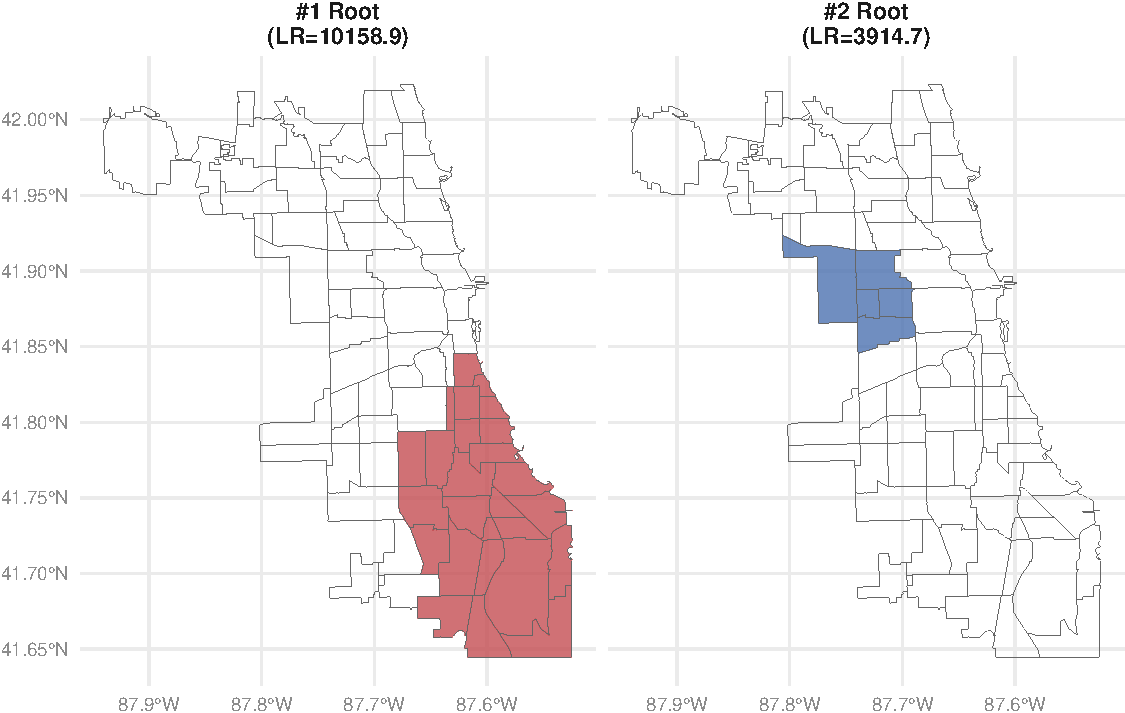
\includegraphics[width=0.9\linewidth]{treeSS_files/figure-latex/chi-plot-top2-1} 

}

\caption{Top-2 distinct tree-spatial clusters in Chicago per Cançado et al. (2025), Section 5.1.1: primary cluster (left) and the highest-LR distinct secondary cluster (right).}\label{fig:chi-plot-top2}
\end{figure}

\hypertarget{road-traffic-collisions-in-london-2022}{%
\subsection{Road traffic collisions in London, 2022}\label{road-traffic-collisions-in-london-2022}}

\texttt{london\_collisions} records all police-reported road collisions in the 33
London boroughs in 2022 (UK STATS19), classified by a tree combining
lighting condition, road type, and junction type. The tree is small (81
nodes), the geography is small (33 boroughs), and the dataset illustrates
the binomial model: each collision is classified as \emph{slight} or
\emph{serious-or-fatal}, and the binomial scan asks where the \emph{proportion}
serious-or-fatal departs from the citywide baseline.

\begin{verbatim}
data(london_collisions)
data(london_tree)
data(london_boroughs_map)

result_ldn <- treespatial_scan(
  cases       = london_collisions$cases,
  population  = london_collisions$population,
  region_id   = london_collisions$region_id,
  x           = london_collisions$x,
  y           = london_collisions$y,
  node_id     = london_collisions$node_id,
  tree        = london_tree,
  max_pop_pct = 0.40,
  nsim        = 999, seed = 2022, n_cores = 4L,
  model       = "poisson"
)
print(result_ldn)
#> Tree-Spatial Scan Statistic
#> -------------------------------------------------- 
#> Total population: 21357 
#> Number of regions: 33 
#> Number of tree nodes: 81 
#> Monte Carlo simulations: 999 
#> 
#> Most likely cluster:
#>   Tree node: Daylight | One way street 
#>   Leaf IDs: Daylight | One way street | 19, Daylight | One way
#>             street | Crossroads, Daylight | One way street |
#>             Junction with more than four arms (not
#>               roundabout),
#>             Daylight | One way street | Not at junction or
#>             within 20 metres, Daylight | One way street | T or
#>             staggered junction, Daylight | One way street |
#>             unknown (self reported), Daylight | One way
#>               street |
#>             Using private drive or entrance
#> 
#>   Regions: 33, 6, 19, 18, 21, 32, 12, 28, 11
#> 
#>   Number of regions: 9 
#>   Cases in (zone, branch): 583 
#>   Expected: 372.09 
#>   Population: 7070 
#>   Relative risk: 1.5668 
#>   Log-LR: 83.703 
#>   P-value: 0.001
\end{verbatim}

The cluster identifies a contiguous group of outer boroughs with elevated
collisions on dark, unlit single-carriageway roads at non-signalized
junctions -- a road-engineering pattern that pure-spatial scans on raw
collision counts would miss because total collisions are dominated by
central, traffic-heavy boroughs. Figure \ref{fig:ldn-plot-primary} shows
the primary cluster; Figure \ref{fig:ldn-plot-top2} shows the top two
distinct clusters per \citet{cancado2025}, Section 5.1.1.

\begin{verbatim}
mlc_ldn <- result_ldn$most_likely_cluster
ldn_lookup <- unique(london_collisions[, c("region_id", "borough")])
cr_ldn_1 <- merge(
  get_cluster_regions(result_ldn, n_clusters = 1L, overlap = FALSE),
  ldn_lookup, by = "region_id"
)
ldn_p1 <- left_join(london_boroughs_map, cr_ldn_1,
                    by = c("NAME" = "borough"))

ggplot(ldn_p1) +
  geom_sf(aes(fill = factor(cluster)), color = "gray40",
          linewidth = 0.15, alpha = 0.80) +
  scale_fill_manual(
    values   = c("1" = "#C44E52"), na.value = "gray95",
    na.translate = FALSE,
    labels   = paste0(mlc_ldn$node_id, " (",
                      length(mlc_ldn$region_ids), " boroughs)"),
    name     = "Cluster"
  ) +
  labs(subtitle = sprintf("LR = %.1f, p = %s | %d collisions (expected %.1f)",
                          mlc_ldn$llr,
                          format.pval(result_ldn$pvalue, digits = 3),
                          mlc_ldn$cases, mlc_ldn$expected)) +
  theme_minimal(base_size = 13) +
  theme(plot.subtitle = element_text(color = "gray35", size = 11),
        axis.title    = element_blank(),
        axis.text     = element_text(color = "gray55", size = 9))
\end{verbatim}

\begin{figure}

{\centering 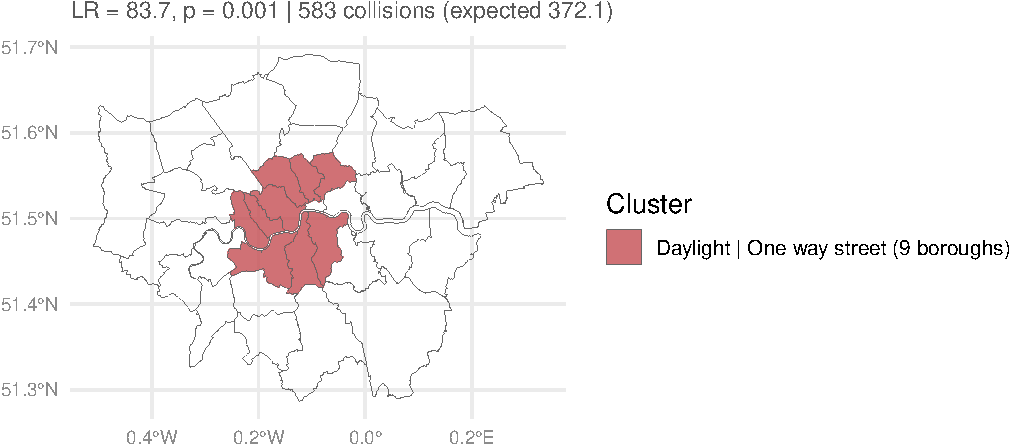
\includegraphics[width=0.9\linewidth]{treeSS_files/figure-latex/ldn-plot-primary-1} 

}

\caption{Most likely tree-spatial cluster in London road collisions, 2022.}\label{fig:ldn-plot-primary}
\end{figure}

\begin{verbatim}
cr_ldn_2 <- merge(
  get_cluster_regions(result_ldn, n_clusters = 2L, overlap = TRUE),
  ldn_lookup, by = "region_id"
)
ldn_p2 <- left_join(london_boroughs_map, cr_ldn_2,
                    by = c("NAME" = "borough"))

ggplot(ldn_p2[!is.na(ldn_p2$panel), ]) +
  geom_sf(aes(fill = factor(cluster)), color = "gray40",
          linewidth = 0.12, alpha = 0.80) +
  scale_fill_manual(values = c("1" = "#C44E52", "2" = "#4C72B0"),
                    na.value = "gray95", na.translate = FALSE) +
  facet_wrap(~ panel, nrow = 1L,
             labeller = labeller(panel = function(x) {
               vapply(x, function(s) {
                 parts <- strsplit(s, "\n", fixed = TRUE)[[1]]
                 wrapped <- vapply(parts, function(p)
                   paste(strwrap(p, width = 32), collapse = "\n"),
                   character(1L))
                 paste(wrapped, collapse = "\n")
               }, character(1L))
             })) +
  theme_minimal(base_size = 12) +
  theme(strip.text = element_text(face = "bold", size = 10),
        axis.title = element_blank(),
        axis.text  = element_text(color = "gray55", size = 9),
        legend.position = "none")
\end{verbatim}

\begin{figure}

{\centering 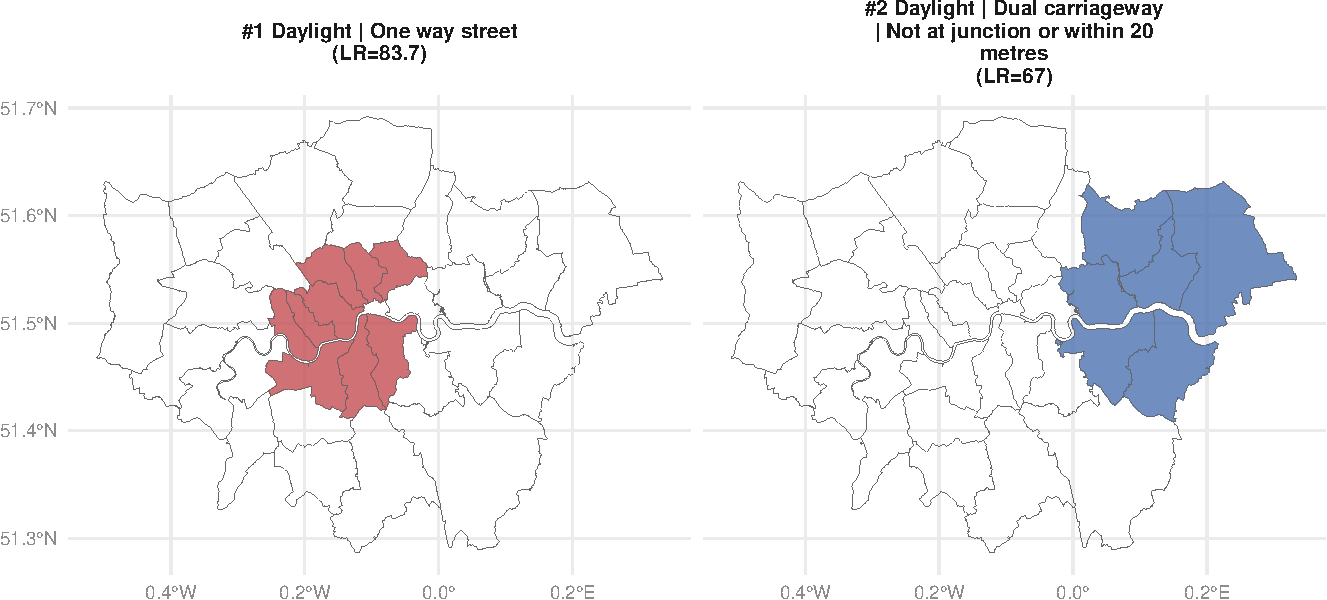
\includegraphics[width=0.9\linewidth]{treeSS_files/figure-latex/ldn-plot-top2-1} 

}

\caption{Top-2 distinct tree-spatial clusters in London per Cançado et al. (2025), Section 5.1.1: primary cluster (left) and the highest-LR distinct secondary cluster (right).}\label{fig:ldn-plot-top2}
\end{figure}

For comparison, Figure \ref{fig:ldn-plot-iter} shows the result of the
\emph{iterative} scan procedure, in which the data are conditioned on each
detected cluster before a fresh Monte Carlo test for the next, with
Holm--Bonferroni correction across iterations. The two procedures answer
different questions: the \citet{cancado2025} filter ranks all (zone, branch)
pairs found by a single scan and selects the most distinct, while the
iterative procedure performs a sequence of independent significance tests.
Both are valid; the iterative procedure tends to detect smaller numbers
of more strongly significant clusters.

\begin{verbatim}
iter_ldn <- iterative_scan(
  cases       = london_collisions$cases,
  population  = london_collisions$population,
  region_id   = london_collisions$region_id,
  x           = london_collisions$x,
  y           = london_collisions$y,
  node_id     = london_collisions$node_id,
  tree        = london_tree,
  max_pop_pct = 0.40,
  max_iter    = 4L, alpha = 0.05,
  nsim        = 999, seed = 2022, n_cores = 4L,
  verbose     = FALSE
)
print(iter_ldn)
#> Iterative Scan
#> -------------------------------------------------- 
#> Scan type: treespatial 
#> Iterations performed: 4 
#> Alpha: 0.05   (applied to Holm-Bonferroni adjusted p-values)
#> 
#> Significant clusters after Holm-Bonferroni: 4 of 4
#> 
#> All iterations:
#>  iteration
#>          1
#>          2
#>          3
#>          4
#>                                                            node_id
#>                                          Daylight | One way
#>                                            street
#>  Daylight | Dual carriageway | Not at junction or within 20
#>    metres
#>  Daylight | Dual carriageway | Not at junction or within 20
#>    metres
#>                                          Darkness | One way
#>                                            street
#>  n_regions cases expected population       rr      llr pvalue
#>          9   583 372.0878       7070 1.566834 83.70304  0.001
#>          6   290 147.7099       3356 1.963308 66.97201  0.001
#>          6   242 129.1661       4244 1.873557 52.31804  0.001
#>          9   288 175.7917       7376 1.638302 51.43052  0.001
#>  pvalue_adjusted significant
#>            0.004        TRUE
#>            0.004        TRUE
#>            0.004        TRUE
#>            0.004        TRUE
\end{verbatim}

\begin{verbatim}
n_iter <- iter_ldn$n_iter
if (n_iter > 0) {
  cr_iter <- merge(
    get_cluster_regions(iter_ldn, n_clusters = n_iter, overlap = TRUE),
    ldn_lookup, by = "region_id"
  )
  ldn_iter_p <- left_join(london_boroughs_map, cr_iter,
                          by = c("NAME" = "borough"))
  pal_iter <- c("#C44E52", "#4C72B0", "#55A868",
                "#8172B2")[seq_len(n_iter)]
  names(pal_iter) <- as.character(seq_len(n_iter))

  ldn_iter_p <- left_join(london_boroughs_map, cr_iter,
                          by = c("NAME" = "borough"))
  pal_iter <- c("#C44E52", "#4C72B0", "#55A868",
                "#8172B2")[seq_len(n_iter)]
  names(pal_iter) <- as.character(seq_len(n_iter))

  ggplot(ldn_iter_p[!is.na(ldn_iter_p$panel), ]) +
    geom_sf(aes(fill = factor(cluster)), color = "gray40",
            linewidth = 0.12, alpha = 0.80) +
    scale_fill_manual(values = pal_iter,
                      na.value = "gray95", na.translate = FALSE) +
    facet_wrap(~ panel, nrow = 2L,
               labeller = labeller(panel = function(x) {
                 vapply(x, function(s) {
                   parts <- strsplit(s, "\n", fixed = TRUE)[[1]]
                   wrapped <- vapply(parts, function(p)
                     paste(strwrap(p, width = 38), collapse = "\n"),
                     character(1L))
                   paste(wrapped, collapse = "\n")
                 }, character(1L))
               })) +
    theme_minimal(base_size = 12) +
    theme(strip.text = element_text(face = "bold", size = 10),
          axis.title = element_blank(),
          axis.text  = element_text(color = "gray55", size = 9),
          legend.position = "none")
} else {
  message("Iterative scan returned no significant clusters at alpha = 0.05.")
}
\end{verbatim}

\begin{figure}

{\centering 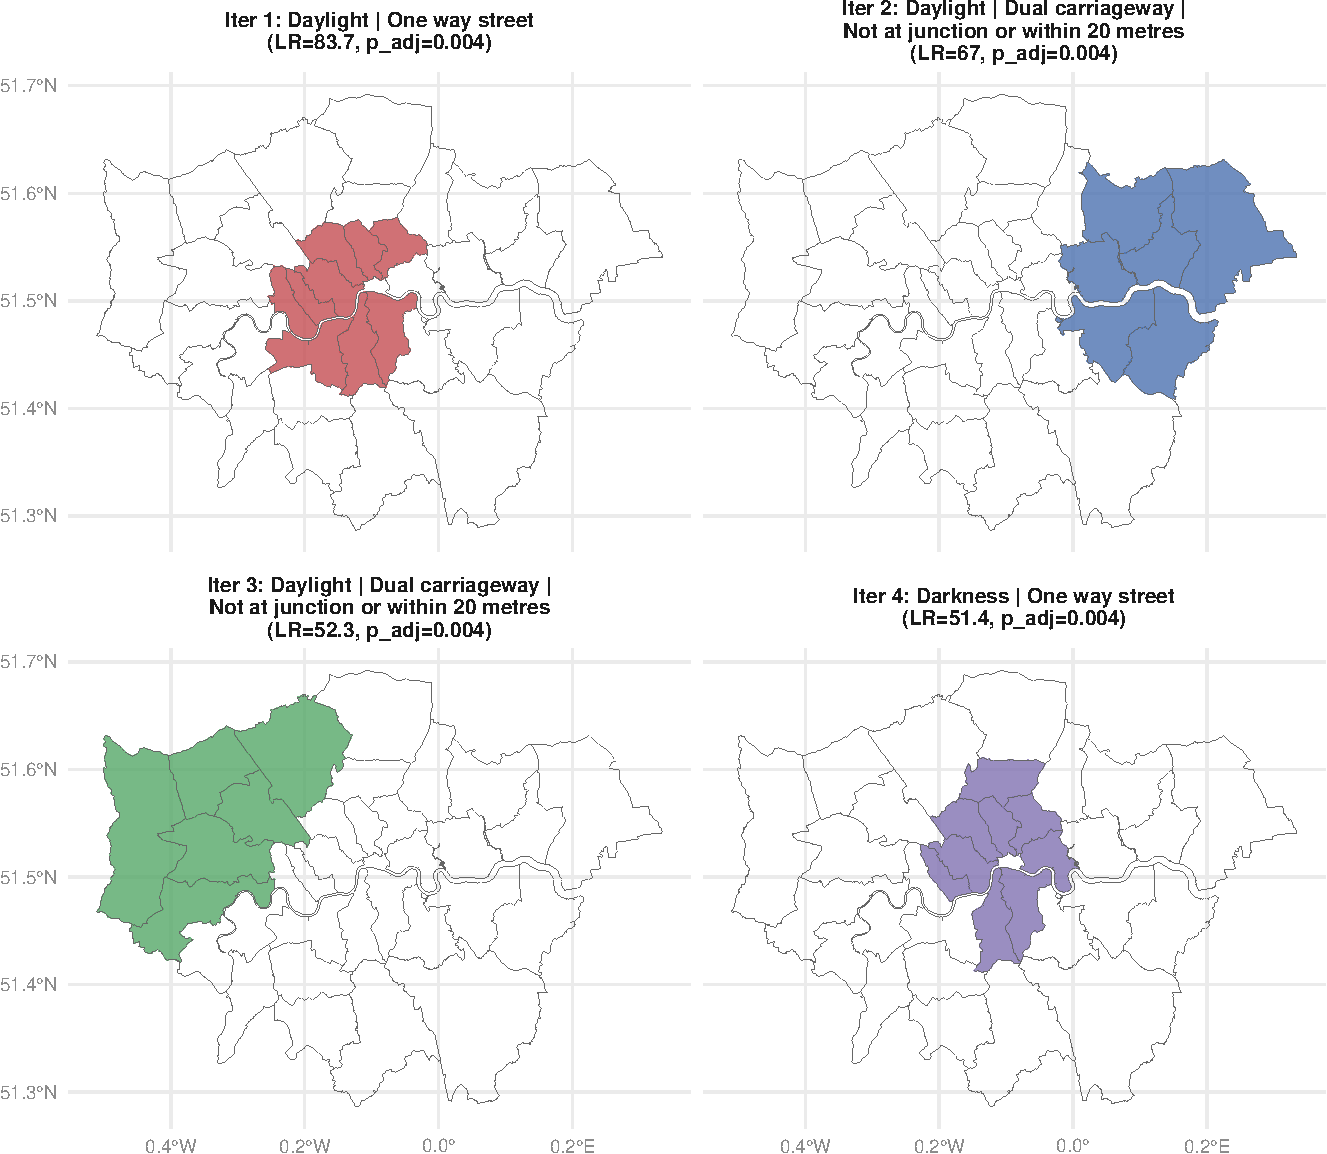
\includegraphics[width=0.9\linewidth]{treeSS_files/figure-latex/ldn-plot-iter-1} 

}

\caption{Iterative scan on London collisions: each cluster is detected after conditioning the data on those previously detected, with Holm--Bonferroni correction across iterations.}\label{fig:ldn-plot-iter}
\end{figure}

A complete annotated workflow with the iterative variant is shipped at
\texttt{system.file("examples",\ "example\_london.R",\ package\ =\ "treeSS")}.

\hypertarget{sec-implementation}{%
\section{Implementation and performance}\label{sec-implementation}}

\hypertarget{architecture}{%
\subsection{Architecture}\label{architecture}}

R orchestrates and validates; C++ does the heavy lifting. The R code
(approximately 1,800 lines across 13 files) handles input normalization,
tree validation, zone construction, output formatting, S3 methods, and
all post-processing. Three Rcpp-exported functions in
\texttt{src/treescan\_core.cpp} (\textasciitilde700 lines of C++) handle the inner loop:

\begin{itemize}
\tightlist
\item
  \texttt{mc\_treespatial\_cpp()} -- Monte Carlo for the tree-spatial scan;
\item
  \texttt{mc\_spatial\_cpp()} -- Monte Carlo for the circular scan;
\item
  \texttt{mc\_treescan\_cpp()} -- Monte Carlo for the tree scan.
\end{itemize}

Each takes the prepared inputs (a leaf-by-region case matrix, the zone
membership matrix, the tree structure, and per-tree-node case rollups) and
returns the simulated null distribution along with the observed
log-likelihood ratio.

The likelihood-ratio evaluation for all (zone, branch) pairs is vectorized
as a single matrix multiplication: \(\mathbf{C}_z = \mathbf{F} \mathbf{Z}^\top\),
where \(\mathbf{F}\) is the \(|T| \times m\) matrix of branch case rollups and
\(\mathbf{Z}\) is the \(|\mathcal{Z}| \times m\) binary zone-membership matrix.
This avoids an explicit double loop over zones and branches in the inner
Monte Carlo iteration.

\hypertarget{complexity-and-scaling}{%
\subsection{Complexity and scaling}\label{complexity-and-scaling}}

For preprocessing, building the family of circular zones requires
\(O(m \log m)\) work per center (sorting other regions by distance) and
produces \(O(m^2)\) candidate zones, capped by \texttt{max\_pop\_pct}. The tree
rollup is linear in the tree size, \(O(|T|)\). The Monte Carlo loop runs
\texttt{nsim} independent replicates, each of which costs \(O(|T| \cdot |\mathcal{Z}|)\)
floating-point operations dominated by the matrix multiply. The package
holds two matrices in memory: the leaf-by-region case matrix
(\(O(\ell \cdot m)\)) and the zone-membership matrix
(\(O(|\mathcal{Z}| \cdot m)\)). For the largest dataset shipped
(\texttt{chicago\_crimes}, \(m = 77\), \(|T| = 2841\), \(\ell \approx 1900\)), peak
memory is well under 1 GB.

\hypertarget{wall-clock-benchmarks}{%
\subsection{Wall-clock benchmarks}\label{wall-clock-benchmarks}}

Table \ref{tab:bench} reports indicative wall-clock times for the three
shipped datasets at \texttt{nsim\ =\ 999} on a typical multicore laptop. The
parallel column uses 4 OpenMP threads.

\begin{table}

\caption{\label{tab:bench}Indicative wall-clock times for nsim = 999. London is small enough that thread-startup overhead dominates.}
\centering
\begin{tabular}[t]{lrrlll}
\toprule
Dataset & Regions & Tree nodes & Serial (s) & 4 threads (s) & Speedup\\
\midrule
rj\_mortality & 89 & 622 & \textasciitilde{}120 & \textasciitilde{}30 & \textasciitilde{}4x\\
chicago\_crimes & 77 & 2841 & \textasciitilde{}480 & \textasciitilde{}110 & \textasciitilde{}4-5x\\
london\_collisions & 33 & 81 & \textasciitilde{}5 & \textasciitilde{}2 & \textasciitilde{}2-3x\\
\bottomrule
\end{tabular}
\end{table}

The Chicago benchmark is the dominant cost in the test suite of the
package and the only one for which we recommend \texttt{nsim\ =\ 999} with
\texttt{n\_cores\ =\ 4L} rather than the serial path. The \textbf{treeSS} Rmarkdown
vignette runs end-to-end in well under ten minutes on a 2024 laptop
using \texttt{n\_cores\ =\ 4}.

\hypertarget{validation}{%
\subsection{Validation}\label{validation}}

The package ships 48 unit tests covering input normalization, tree
validation, zone construction, Poisson and binomial likelihood ratios on
small toy inputs with known analytical answers, parallel-vs-serial
equivalence at \texttt{n\_cores\ =\ 1}, and full reproducibility under fixed seeds.
Continuous integration on GitHub Actions exercises the package on
Linux, macOS and Windows with R-release and R-devel.

\hypertarget{limitations}{%
\subsection{Limitations}\label{limitations}}

Three limitations are worth flagging.

\begin{itemize}
\tightlist
\item
  \textbf{Circular zones inherit Kulldorff's elongation bias.} When the true
  cluster has irregular shape, circular zones will either include
  uninvolved regions or split the cluster across several zones. The
  package does not yet support irregularly shaped zones, although this
  is a planned extension. Users with strong prior belief in elongated
  clusters can pre-filter the data spatially.
\item
  \textbf{Degenerate trees.} A tree consisting of a single node coincides with
  no tree at all and reduces the tree-spatial scan to the circular scan.
  We recommend using \texttt{circular\_scan()} directly in that case.
\item
  \textbf{Small \texttt{nsim}.} Setting \texttt{nsim\ \textless{}\ 99} produces a \(p\)-value resolution
  coarser than \(0.01\) and is discouraged. The default of \(999\) gives a
  resolution of \(0.001\) with negligible runtime overhead at typical
  problem sizes.
\end{itemize}

\hypertarget{sec-comparison}{%
\section{Comparison with related packages}\label{sec-comparison}}

\begin{table}

\caption{\label{tab:related}treeSS in the landscape of scan-statistic software.}
\centering
\begin{tabular}[t]{llll}
\toprule
Tool & Scan type & Implementation & On CRAN\\
\midrule
treeSS & tree-spatial, tree, circular & R + C++ (Rcpp, OpenMP) & yes (this paper)\\
scanstatistics & space-time anomaly detection & R & yes\\
rsatscan & inherits from SaTScan & R wrapper around binary & yes\\
SpatialEpi & circular Kulldorff & R & yes\\
SaTScan & circular, elliptic, space-time & C++ standalone & no\\
\addlinespace
TreeScan & tree-only, tree-time & C++ standalone & no\\
\bottomrule
\end{tabular}
\end{table}

\CRANpkg{SpatialEpi} provides Kulldorff's circular spatial scan in pure R.
For purely spatial problems on small to moderate study areas it is a
mature and convenient choice; \textbf{treeSS} does not aim to replace it.
However, on the spatial-only subset of problems, \texttt{treeSS::circular\_scan()}
returns equivalent point estimates and Monte Carlo \(p\)-values, with the
benefit of the OpenMP-parallelized C++ inner loop for large \texttt{nsim}.

\CRANpkg{scanstatistics} addresses \emph{space-time} anomaly detection
\citep{scanstatistics}, a different problem in which the tree dimension is
absent. The two packages are complementary rather than competitive.

\CRANpkg{rsatscan} is a thin R wrapper around the SaTScan binary
\citep{satscan}; users must install SaTScan separately and the package writes
input files to disk, calls the binary, and parses the output. SaTScan is
the reference implementation of Kulldorff's spatial and space-time scans
and offers shape options (elliptic, irregular) that \textbf{treeSS} does not.
However, SaTScan does not implement a tree-spatial scan: there is no way
to pass a tree of categories alongside the spatial inputs.

The standalone TreeScan software \citep{treescan} implements the tree-based
scan and the tree-time scan but, like SaTScan, does not perform a joint
search over space and tree. There is no R interface to TreeScan.

To our knowledge \textbf{treeSS} is therefore the first implementation of any
kind -- R or otherwise -- of the tree-spatial scan statistic of
\citet{cancado2025}.

\hypertarget{sec-discussion}{%
\section{Discussion}\label{sec-discussion}}

We have described \textbf{treeSS}, an R package that implements the
tree-spatial scan statistic of \citet{cancado2025} alongside the classical
circular spatial scan and the tree-based scan, under a unified parallel
vector input contract. The package fills a concrete gap in the R
ecosystem: no previous CRAN package implements a scan that searches
jointly over circular spatial zones and branches of a hierarchical
classification tree. The core search is implemented in C++ via Rcpp and
optionally parallelized with OpenMP, and the package ships three real
datasets that allow users to run a complete workflow without preparing
data themselves.

We see three priorities for future work. First, \textbf{irregular zones}: the
elongation bias of circular zones is well-documented and a Duczmal-style
graph-cut zone family would extend \textbf{treeSS} to that setting with no
change to the methodology of \citet{cancado2025} -- only the
zone-construction step. Second, a \textbf{space-time-tree extension}:
combining the tree dimension of \citet{kulldorff2003} with the space-time
dimension of \citet{scanstatistics} is a natural three-way generalization
relevant to outbreak surveillance. Third, \textbf{native \texttt{sf} integration}:
currently users supply centroids as \texttt{(x,\ y)} columns; accepting an
\texttt{sf::sf} object directly would make the package more idiomatic for
modern spatial-R workflows.

In its current form \textbf{treeSS} is, we believe, ready to support applied
work. The Rio de Janeiro reproduction in Section \ref{sec-example} and
the Chicago and London applications in Section \ref{sec-applications}
illustrate the breadth of problems for which a tree-spatial perspective
gives non-trivial signal that pure-spatial or pure-tree analyses miss.
We hope the package will lower the barrier to such analyses and
encourage the broader adoption of joint scan statistics in
surveillance practice.

\hypertarget{acknowledgements}{%
\section*{Acknowledgements}\label{acknowledgements}}
\addcontentsline{toc}{section}{Acknowledgements}

A.L.F.C., G.S.O. and L.H.D. acknowledge the support of CNPq and CAPES.
A.V.C.Q. thanks the maintainers of the open-source R ecosystem on which
this work is built, in particular the authors of \CRANpkg{Rcpp},
\CRANpkg{SpatialEpi}, \CRANpkg{geobr} and the \textbf{rjtools} team. The
DATASUS, IBGE, City of Chicago, and UK Department for Transport open data
programs made the applied examples in this paper possible.

\bibliography{treeSS.bib}

\address{%
Allan Quadros\\
Department of Management, University of North Florida\\%
1 UNF Drive\\ Jacksonville, FL 32224, USA\\
%
\url{https://github.com/allanvc}\\%
\textit{ORCiD: \href{https://orcid.org/0000-0003-3250-5380}{0000-0003-3250-5380}}\\%
\href{mailto:allanvcq@gmail.com}{\nolinkurl{allanvcq@gmail.com}}%
}

\address{%
André L. F. Cançado\\
Department of Statistics, University of Brasília\\%
Campus Universitário Darcy Ribeiro, Asa Norte\\ Brasília, DF, 70910-900, Brazil\\
%
%
\textit{ORCiD: \href{https://orcid.org/0000-0002-7019-8521}{0000-0002-7019-8521}}\\%
\href{mailto:cancado@unb.br}{\nolinkurl{cancado@unb.br}}%
}

\address{%
Geiziane S. Oliveira\\
Federal University of Minas Gerais\\%
Av. Antônio Carlos 6627\\ Belo Horizonte, MG, 31270-901, Brazil\\
%
%
%
\href{mailto:geiziane@ufmg.br}{\nolinkurl{geiziane@ufmg.br}}%
}

\address{%
Luiz H. Duczmal\\
Federal University of Minas Gerais\\%
Av. Antônio Carlos 6627\\ Belo Horizonte, MG, 31270-901, Brazil\\
%
%
%
\href{mailto:duczmal@ufmg.br}{\nolinkurl{duczmal@ufmg.br}}%
}
